\documentclass[a4paper]{article}\usepackage[english]{babel}
\usepackage[utf8x]{inputenc}
\usepackage{amsmath}
\usepackage{hyperref}
\usepackage{graphicx}
\usepackage[colorinlistoftodos]{todonotes}
\usepackage[]{mcode}
\usepackage{placeins}
\title{Using a Lock-In amplifier to determine filters from High Pass, Low Pass and Band Pass circuits }
\author{Aaron Kebede}
\date{\today}
\begin{document}
\maketitle
\begin{abstract}

This report provides insight into the analysis of R-C Circuits using signal generators. We study circuits in three steps. First, we study a very simple circuit just consisting of a resistor, a capacitor element, and a signal generator. The signal generator generates a current with a specific frequency which we can then vary to study the effects on the other circuit elements. Second, we create a virtual instrument(using LabVIEW) program to automate alteration of the frequency and third, we add a lock-in amplifier in the circuit to extract all the signals and automate our process of collecting the data. We find that for large frequencies, the phase shift is slightly negatively correlated with the frequency while the amplitude has a strong positive correlation. The data, its analysis, and full plots are available at \url{https://220.kebede.org}

\end{abstract}

\section{Introduction}

Included in this report are details of the method, graphs, results, error analysis, discussions and conclusions of results. We record data and analyze it to find correlations between signals sent from the signal generator and the feedback from the circuit recorded in different sets.  
\newline
\newline
We performed our data collection in three steps:
\newline
\begin{Steps}
 \item{1. We set up a circuit with a variable resistor, variable capacitor, and  an function generator. We varied the signal on the function generator and then recorded the data \textbf{by hand} on an excel sheet.} \newline{}
 \item{2. We then created a LabVIEW program to automate the signals that were being generated. } \newline{}
 \item{3. }
 
\end{Steps}

\begin{figure}
  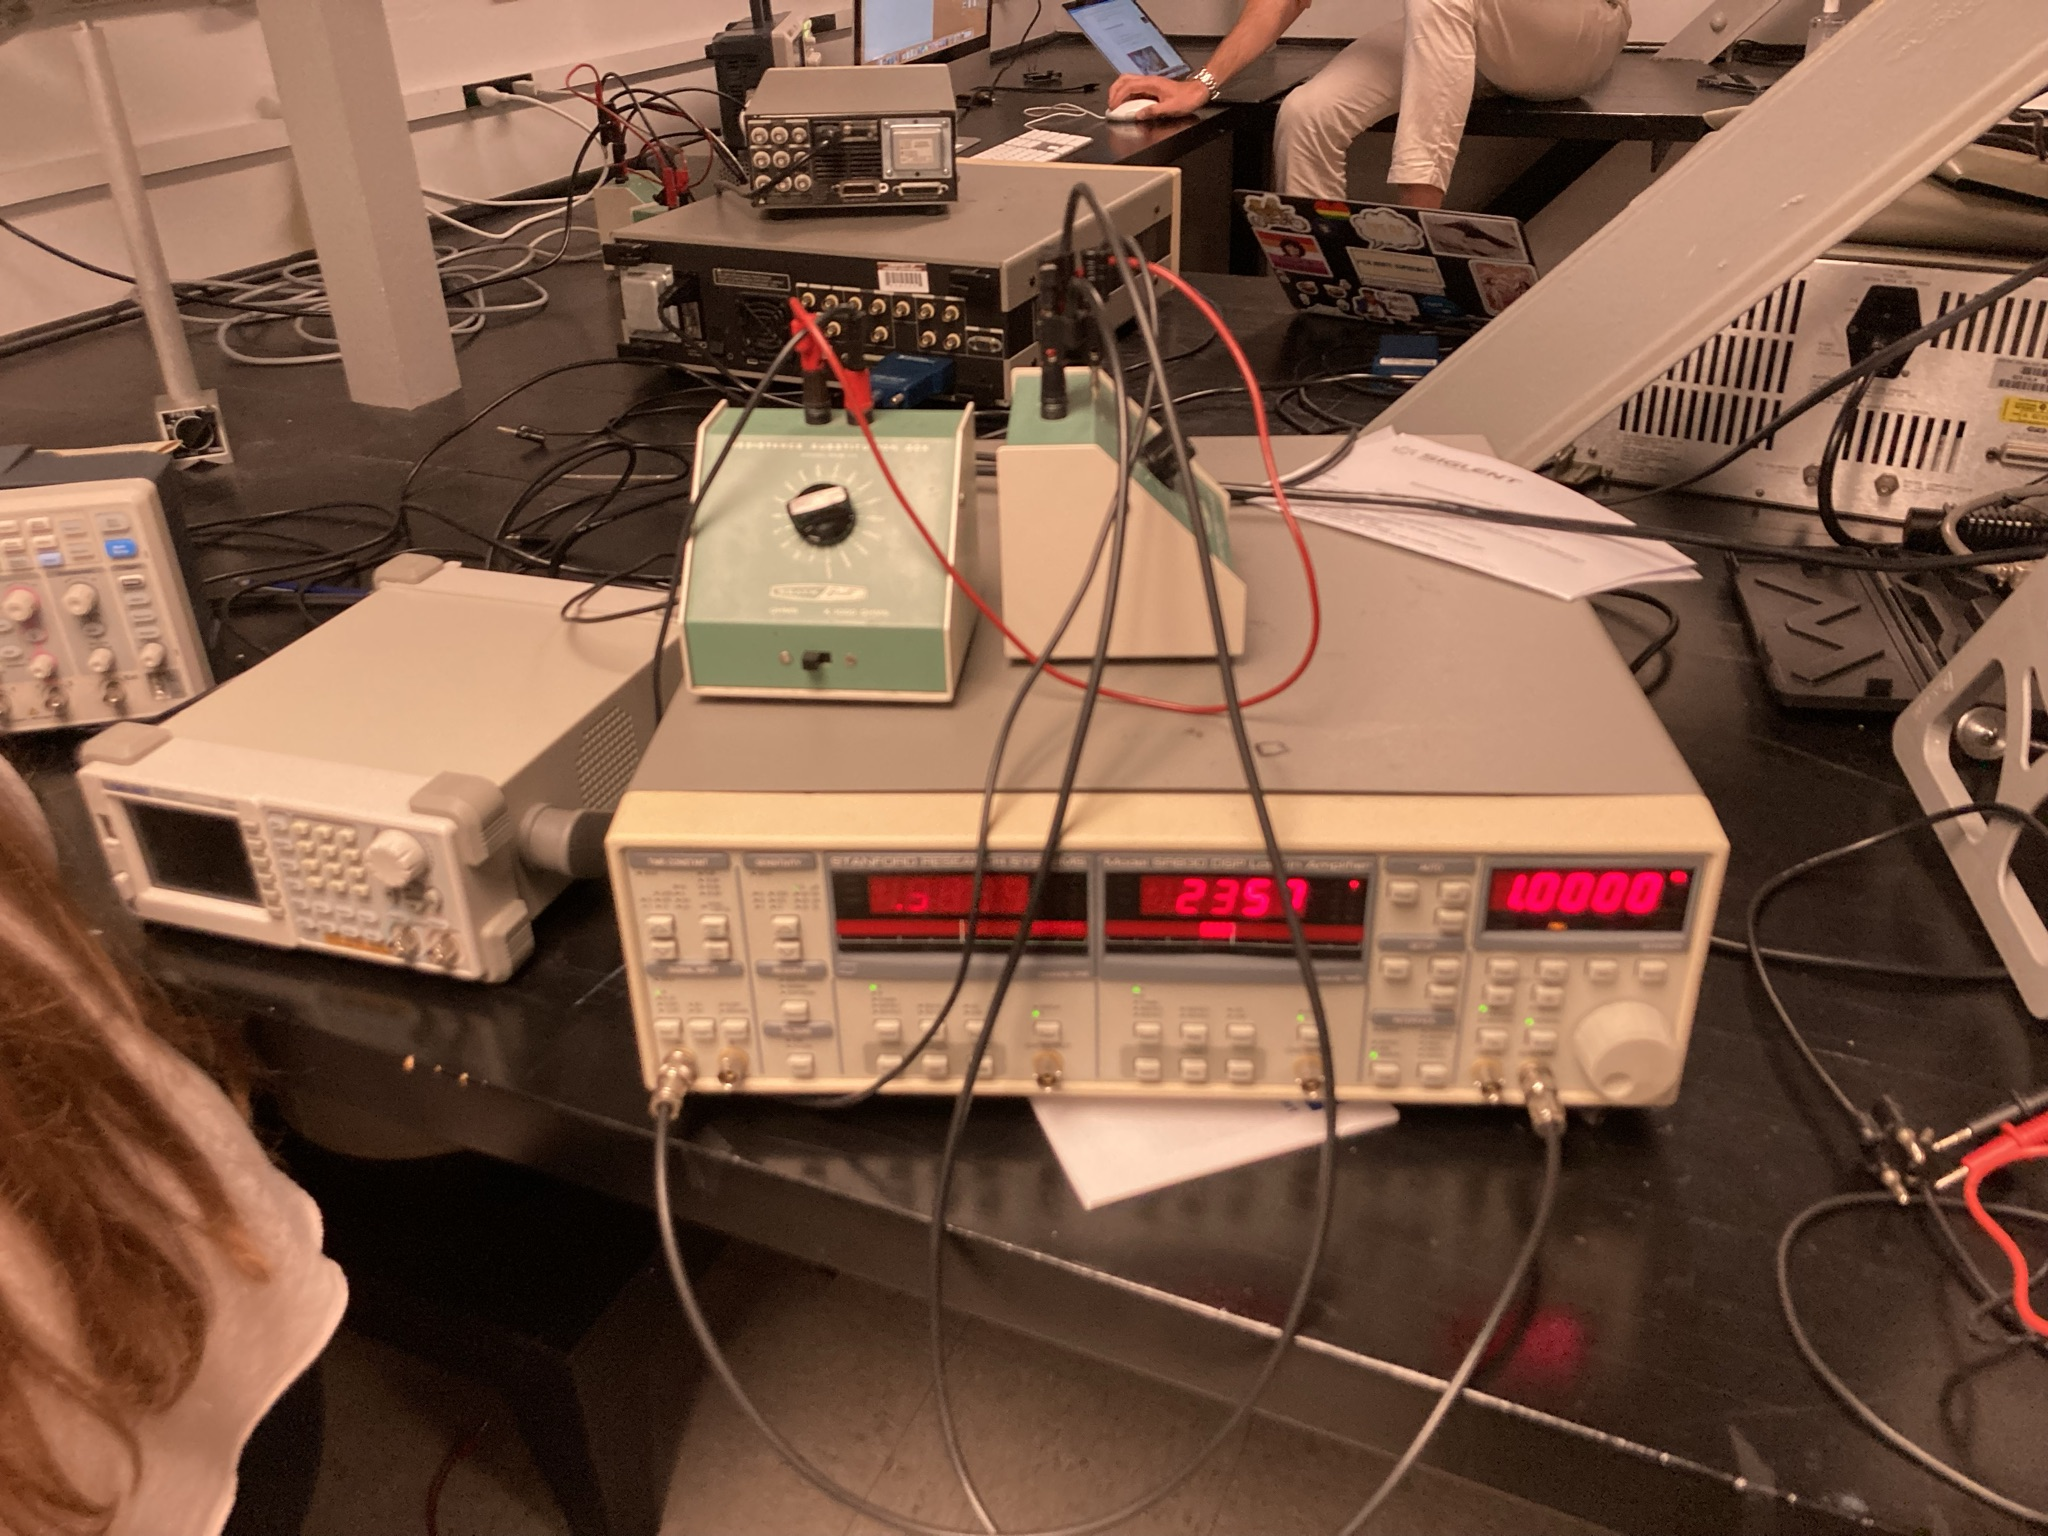
\includegraphics[width=\linewidth]{images/lab/setup.JPEG}
  \caption{Our lab setup}
  \label{fig:boat1}
\end{figure}

\end{document}